\chapter{Introduction}
\label{chapter:intro}


\section{Background}
Image generation is a process that involves utilizing computer algorithms and models to create new images. This intricate process typically incorporates mathematical and statistical methods, along with extensive training data, enabling computers to generate images with diverse visual features and structures. By leveraging existing data and models, the computational system can produce highly realistic images.

In practical applications, components can be categorized into "old components," which have ample normal and defective samples, and "new components," where defective samples may be insufficient or lacking. It is crucial to note that the types of defects for both new and old components are identical, as detailed in Table 1.1.
\renewcommand{\arraystretch}{1.5} % 调整行高
\setlength{\tabcolsep}{10pt} % 调整列间距

\begin{table}[h]
    \centering
    \begin{tabular}{lll} \hline  
         &  Normal& Defect\\ \hline  
         New component&  Numerous& Numerous\\ \hline  
         Old componet&Numerous&Several or None\\ \hline 
    \end{tabular}
    \caption{The types of defects for both new and old components}
    \label{tab:my_label}
\end{table}
Traditional models exhibit suboptimal performance in generating defects for new components. Consequently, our research focuses on designing a more effective model structure for generating defect features when only defective samples from old components are available.

The challenge lies in innovatively addressing the deficiency of defect samples for new components, thereby enhancing the model's ability to generate realistic and diverse defect features. Through this research, we aim to contribute to the advancement of image generation techniques, particularly in scenarios where limited or no defect data is available for new components.


\section{Motivation}
Taiwan's Printed Circuit Board (PCB) industry holds the leading position in global market share. For PCB manufacturers, the yield rate of circuit boards is crucial; a poor yield rate not only increases costs but also damages corporate reputation. Some manufacturers employ Artificial Intelligence (AI) to develop "Defect Detection" systems, significantly enhancing product quality and inspection efficiency. However, these systems perform poorly in identifying defect types in unseen components, necessitating the use of image generation technology.

Welding is a common technique in industrial manufacturing, involving the connection of electronic components. However, the welding process introduces challenges such as high temperatures, high pressures, and the potential for chemical reactions, making it susceptible to defects. These defects can disrupt the entire manufacturing process or result in subpar quality of the final product. Therefore, the development of imaging techniques capable of generating images of defects in new components becomes crucial.

In the current field of image generation, text-to-image techniques, such as OpenAI's Stable Diffusion\cite{Stable_Diffusion} method, are widely applied. However, in our experiments, the goal is not to generate generalized patterns but rather specific images related to industrial manufacturing. When providing descriptions of our industrial components to ChatGPT, converting them into prompts, and subsequently utilizing Stable Diffusion for image generation, we observed significant discrepancies and even errors in the generated images.

In addressing these challenges, the use of Conditional Diffusion Models(CDMs) demonstrates significant potential, particularly in handling complex variation processes. The distinctive feature of CDMs lies in their ability to generate images with specific features based on different conditions. They not only model common defect characteristics but also generate corresponding defect images based on the characteristics of different components.

The use of CDMs helps overcome the deficiency of defect samples for new components. By learning from existing data, these models can generate a broader range of defect scenarios based on class conditions, to enhance the accuracy of generating defect images. This, in turn, contributes to minimizing disruptions in the entire manufacturing process and preventing a decline in product quality.


\section{Goal}
The PCB dataset used in this study was provided by a collaborative industry partner of our laboratory, and was used previously for defect detection research. In the initial phase of this project, the dataset was used to investigate the generation of "zero-shot" images, and it will be employed as an augmented dataset for defect detection in the subsequent stages of this research.

As shown in Figure 1.1, we present the representation of component groups and defect types. It can be observed that the combination within the "Broke Group3" is not present in this dataset.
\begin{figure}[H]
    \centering
    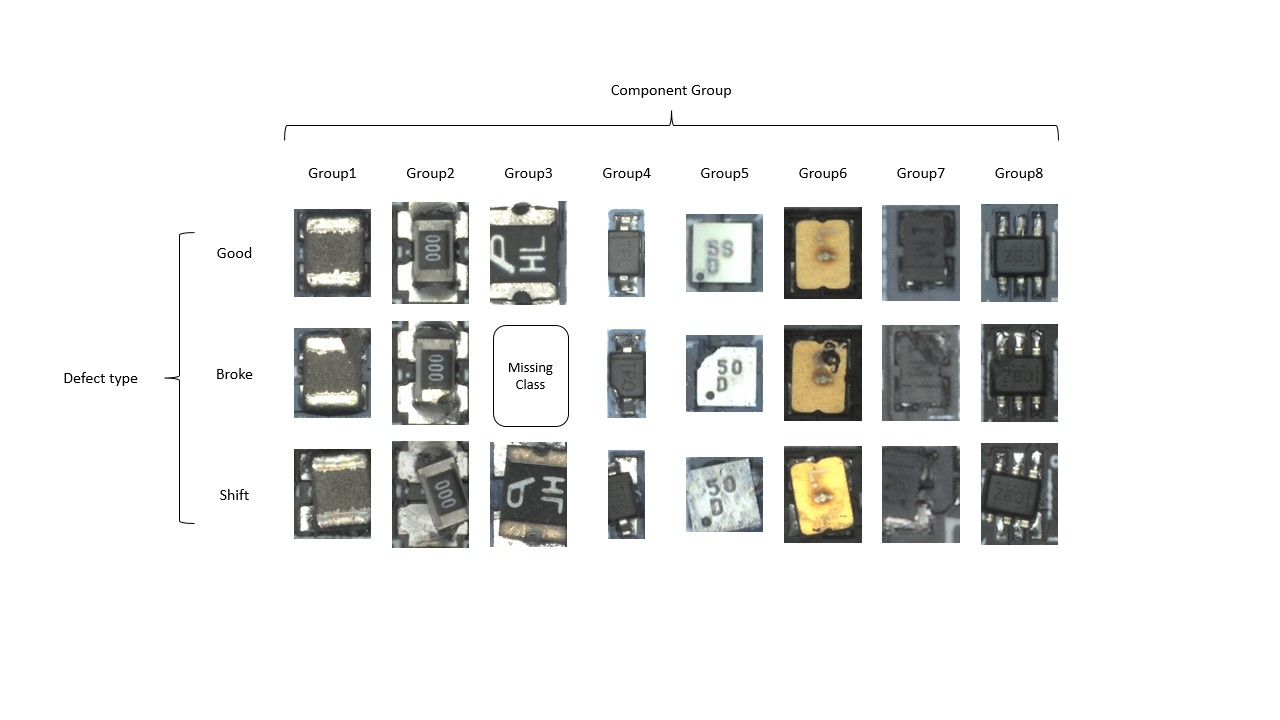
\includegraphics[width=1\linewidth]{Goal.jpg}
    \caption{The representation of component groups and defect types }
    \label{fig:enter-label}
\end{figure}

This study aims to employ an estimation method based on diffusion processes, utilizing a Compositional Class-to-image approach to generate defect images for new components (Broke Group3). The produced new components (Broke Group3) will be integrated into the defect component detection model to enhance the model's generalization ability to unseen images. Additionally, we implement Denoising Diffusion Implicit Models(DDIM)\cite{DDIM} sampling to expedite the generation process. The overarching goal is to provide direction and inspiration for future research in this domain.


\section{Contribution}
The contributions of this thesis are summarized in the following:
\begin{itemize}
    \item We propose a novel class-to-image generation method that reduces training time by eliminating the need for additional text pre-training models, such as CLIP\cite{CLIP}.
    \item Unlike traditional prompts requiring lengthy descriptions, our method does not rely on complex textual inputs yet is capable of producing accurate and exceptional images even in unseen contexts. This approach simplifies the generation process while ensuring both accuracy and diversity in the generated images.
    \item \textbf{Novelty in New Component Defect Generation Model}: Our study pioneers the use of the Compositional Conditional Diffusion method for generating defects in previously unseen new components. This groundbreaking approach represents a new contribution to the field, introducing a unique and innovative model for defect generation.
    \item \textbf{Practical Application Scenarios}: The potential real-world impact of our model, especially in the industrial welding domain, underscores its practical utility. This application-oriented contribution enhances the relevance and applicability of our research in addressing challenges within the welding industry.
\end{itemize}

